\begin{definition}[Submersão]
  Seja $U\subseteq \mathbb{R}^{n}$ aberto, $f:U\to\mathbb{R}^{m}$ é dita \textbf{submersão} no ponto $x\in U$ se $f^{\prime}(x):\mathbb{R}^{m}\to\mathbb{R}^{n}$ é sobrejetiva (ou seja $m\geq n$). 
\end{definition}
\begin{note}
  Note que a composta das submersões é uma submersão.
\end{note}
\begin{example}
  Seja $p:\mathbb{R}^{m}\times\mathbb{R}^{n}\to\mathbb{R}^{n}$ a projeção $p(x,y)=y$.\\
  Note que $p$ é linear, logo $p^{\prime}=p$, assim $p^{\prime}$ é sobrejetiva e portanto uma submersão. 
\end{example}
\begin{example}
  Seja $f:\mathbb{R}^{m}\to\mathbb{R}$ dada por $f(x,y)=\norm{x}^{2}-\norm{y}^{2}$ com $x\in\mathbb{R}^{m-i}$ e $y\in\mathbb{R}^{i}$.\\
  Logo
  \begin{align*}
    f^{\prime}(x,y)\cdot (h,k)=2\left\langle x,h \right\rangle-2\left\langle y,k \right\rangle.
  \end{align*}
  Então, $f^{\prime}\big|_{\mathbb{R}^{m}\setminus\{0\}}$ é submersão, ja que $f^{\prime}(x,y)\neq 0$ para todo $(x,y)\in\mathbb{R}^{m}\setminus\{0\}$. 
\end{example}
\begin{notation}
  Escrevemos $\mathbb{R}^{n+m}=E\oplus F$ com $z=(x,y)$, $x\in E$ e $y\in F$. E as derivadas parciais.
  \begin{align*}
    \partial_{1}f(z_0)&=f^{\prime}(z_0)\big|_{E}:E\to\mathbb{R}^{n}.\\
    \partial_{2}f(z_0)&=f^{\prime}(z_0)\big|_{F}:F\to\mathbb{R}^{n}.
  \end{align*}
\end{notation}
\begin{theorem}[Forma local das submersões]
  Sejam $U\subseteq\mathbb{R}^{m+n}$ aberto, $f:U\to\mathbb{R}^{n}$ de classe $C^{k}$ ($k\geq 1$), submersão em $z_0\in U$ (i.é, $f^{\prime}(z_0)$ é sobrejetiva).\\
  Dada uma descomposição $\mathbb{R}^{m+n}=E\oplus F$ com $z_0=(x_0,y_0)$ tal que $\partial_{2}f(z_0):F\to\mathbb{R}^{n}$ é um isomorfismo.\\
  Então exise um difeomorfismo $h:V\times W\to Z$ de classe $C^{k}$, onde
  \begin{itemize}
    \item $V\subseteq E$ é aberto com $x_0\in V$.
    \item $W\subseteq \mathbb{R}^{n}$ é aberto com $f(z_0)\in W$.
    \item $Z\subseteq U$ é aberto com $z_0\in Z$. 
  \end{itemize}
  Tal que $f(h(x,w))=w$ para todo $(x,w)\in V\times W$. 
\end{theorem}
\begin{proof} 
  \begin{center}
    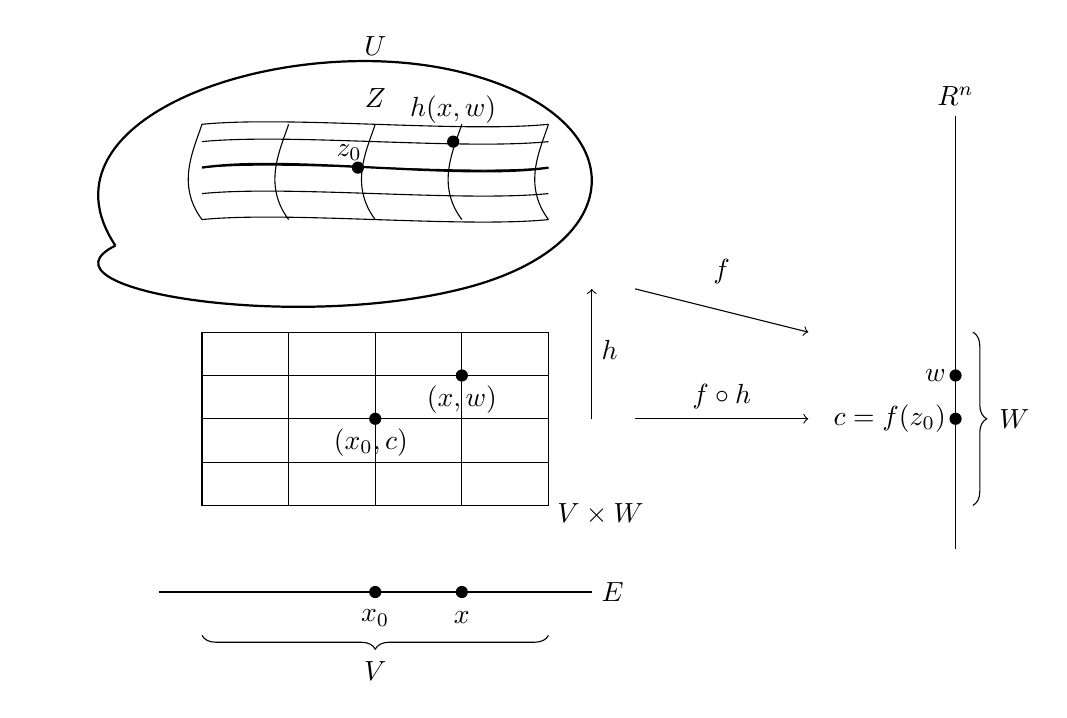
\begin{tikzpicture}[scale=1.1]

% ======================
% REGIÓN SUPERIOR (U)
% ======================

% Contorno tipo "orgánico"
\draw[thick] (-5,1.5) .. controls (-6,3) and (-3,4) .. (-1,3.5)
             .. controls (1,3) and (1,1.5) .. (-1,1)
             .. controls (-3,0.5) and (-6,1) .. (-5,1.5);

\node at (-2,3.8) {$U$};
\node at (-2,3.2) {$Z$};

% "Fibras" (curvas horizontales suaves)
\foreach \y in {1.8,2.1,2.4,2.7,2.9} {
    \draw (-4,\y)
    .. controls (-3,{\y+0.1}) and (-1,{\y-0.1}) ..
    (0,\y);
}

% Fibra destacada (la del punto a)
\draw[thick]
(-4,2.4)
.. controls (-3,2.55) and (-1,2.25) ..
(0,2.4);

% Líneas verticales (estructura tipo producto)
\draw (-3,1.8)
.. controls (-3.3,2.2) and (-3.1,2.6) ..
(-3,2.9);

\draw (-2,1.8)
.. controls (-2.3,2.2) and (-2.1,2.6) ..
(-2,2.9);

\draw (-1,1.8)
.. controls (-1.3,2.2) and (-1.1,2.6) ..
(-1,2.9);

\draw (-4,1.8)
.. controls (-4.3,2.2) and (-4.1,2.6) ..
(-4,2.9);

\draw (0,1.8)
.. controls (-0.3,2.2) and (-0.1,2.6) ..
(0,2.9);


% Punto a
\fill (-1.1,2.7) circle (2pt);
  \node[above] at (-1.1,2.8) {$h(x,w)$};

% Punto izquierda
\fill (-2.2,2.4) circle (2pt);
\node[above] at (-2.3,2.37) {$z_0$};

% ======================
% REGIÓN INFERIOR (V x W)
% ======================

\draw (-4,-1.5) rectangle (0,0.5);
\node at (0.6,-1.6) {$V\times W$};
% Grid
\foreach \x in {-4,-3,-2,-1,0} {
    \draw (\x,-1.5) -- (\x,0.5);
}
\foreach \y in {-1,-0.5,0} {
    \draw (-4,\y) -- (0,\y);
}

% Punto (a1,c)
\fill (-2,-0.5) circle (2pt);
  \node[below] at (-2.05,-0.5) {$(x_0,c)$};

% Punto (x,c)
\fill (-1,0) circle (2pt);
\node[below] at (-1,0) {$(x,w)$};

% Flecha h
\draw[->] (0.5,-0.5) -- (0.5,1);
\node[right] at (0.5,0.3) {$h$};

% ======================
% EJE INFERIOR (R^m)
% ======================

\draw (-4.5,-2.5) -- (0.5,-2.5);
\node[right] at (0.5,-2.5) {$E$};

\fill (-1,-2.5) circle (2pt);
\node at (-1,-2.8) {$x$};
\fill (-2,-2.5) circle (2pt);
\node at (-2,-2.8) {$x_0$};
% Segmento W
\draw[
  decorate,
  decoration={brace, mirror, amplitude=5pt}
]
(-4,-3) -- (0,-3)
node[midway, below=6pt] {$V$};

% ======================
% LADO DERECHO (R^n)
% ======================

\draw (4.7,-2) -- (4.7,3);
\node[above] at (4.7,3) {$\mathbb{R}^n$};

% Segmento W
\draw[
  decorate,
  decoration={brace, mirror, amplitude=5pt}
]
(4.9,-1.5) -- (4.9,0.5)
node[midway, right=6pt] {$W$};

\fill (4.7,-0.5) circle (2pt);
\node[left] at (4.7,-0.5) {$c=f(z_0)$};

\fill (4.7,0) circle (2pt);
\node[left] at (4.7,0) {$w$};

% Flecha f diagonal
\draw[->] (1,1) -- (3,0.5);
\node at (2,1.2) {$f$};

% Flecha horizontal
\draw[->] (1,-0.5) -- (3,-0.5);
\node[above] at (2,-0.5) {$f\circ h$};

\end{tikzpicture}
  
  \end{center}
  Seja $\phi:U\to E\times\mathbb{R}^{n}$ definida por $\phi(x,y)=(x,f(x,y))$.\\
  Note que a derivada de $\phi$ é dada por
  \begin{align*}
    \phi^{\prime}(z_0)\cdot(h,k)=\left( h,\partial_{1}f(z_0)\cdot h+\partial_{2}f(z_0)\cdot k \right),
  \end{align*}
  para todo $(h,k)\in E\oplus F$.\\
  \textbf{Afirmação:} $\phi^{\prime}(z_0)$ é um isomorfimo em $z_0=(x_0,y_0)$.\\
  Precisamos resolver quando $\phi^{\prime}(z_0)\cdot(h,k)=(u,v)$ onde $u\in E$ e $v\in \mathbb{R}^{n}$. Isto é
  \begin{align*}
    \begin{cases}
      h=u, &\text{,} \\
      \partial_{1}f(z_0)\cdot h+\partial_{2}f(z_0)\cdot k=v, &.
    \end{cases}
  \end{align*}
  Subtituindo chegamos a $\partial_{1}f(z_0)\cdot u+\partial_{2}f(z_0)\cdot k=v$. Logo como $\partial_{2}f(z_0)$ é isomorfismo, existe $\left[ \partial_{2}f(z_0) \right]^{-1}$, então
  \begin{align*}
    k=\left[ \partial_{2}f(z_0) \right]^{-1}\left( v-\partial_{1}f(z_0)\cdot h \right).
  \end{align*}
  Logo, temos que $\phi^{\prime}(z_0)$ é sobrejetiva, logo pelo ser transformação linear e as dimenções do $U$ e $E\times\mathbb{R}^{n}$ ser as mesmas, temos que ela é bijetiva, pelo que podemos concluir que $\phi^{\prime}(z_0)$ é um isomorfismo.\\
  Agora, pelo teorema de la aplicação inversa existe um aberto $Z\subseteq U$ tal que $z_0\in Z$, e um aberto $V\times W\subseteq E\times\mathbb{R}^{n}$ com $\phi(z_0)=(x_0,f(z_0))\in V\times W$ tal que $\phi\big|_{Z}:Z\to V\times W$ é difeomorfismo.\\
  Assim, defina $h=\left[ \phi\big|_{Z} \right]^{-1}:V\times W\to Z$ a qual é umm difeomorfismo.
  Além disso, para todo $(x,w)\in V\times W$ temos $f(h(x,w))=w$. 
\end{proof}
